\documentclass[11pt]{article}

\usepackage{amsmath}
\usepackage{amsfonts} 
\usepackage{amsthm}
\usepackage{blkarray}
\usepackage{caption}
\usepackage{enumitem} 
\usepackage{mathtools}
\usepackage{tikz}
\usepackage[top=2cm,bottom=2cm,left=2cm,right=2cm,marginparwidth=1.75cm]{geometry}
\setlength{\parindent}{0cm}
\newcommand{\R}{\mathbb{R}}
\newcommand\simpleGraph[1]{
  \begin{tikzpicture}[every node/.style={circle,draw}]
    \node (a) at (0,1) {};
    \node (b) at (1,1) {};
    \node (c) at (1,0) {};
    \node (d) at (0,0) {};

    \foreach \from/\to in {#1}
      \draw (\from) -- (\to);
  \end{tikzpicture}\hfil
}
\newcommand\itm[1]{\item[\textbf{#1}]}
\newcommand{\incid}{{-}\!{\bullet}\!{-}}
\newcommand{\n}{\vspace{0.3cm}}

\def\lc{\left\lceil}   
\def\rc{\right\rceil}
\def\lf{\left\lfloor}   
\def\rf{\right\rfloor}

\newtheorem{theorem}{Theorem}

\title{\vspace{-1.0cm}MATH 5707 Homework 2}
\author{Fletcher Gornick}
\date{February 14, 2023}

\begin{document}
\maketitle
\begin{itemize}
  \itm{2.1.6} Show that if \(G\) is a tree with \(\Delta \geq k\), then \(G\) has at least \(k\) vertices of degree one.
  \begin{proof}
    From theorems 1.1 and 2.2, we know \(\displaystyle\sum_{v \in V} d_G(v) = 2\varepsilon = 2\nu - 2.\)
    Now we can let \(\ell\) denote the number of vertices with degree 1 in \(G\).  Without loss of generality, let \(v_1\) be our vertex with \(d_G(v_1) \geq k\).  Let the next \(\ell\) vertices \(v_2,v_3,\hdots,v_{\ell + 1}\) have degree 1, and the remaining \(\nu - \ell - 1\) vertices \(v_{\ell+2}, v_{\ell+3}, \hdots, v_{\nu}\) have degree \(\geq 2\).  This gives us the following inequality,
    \[k + \ell + 2(\nu - \ell - 1) \;\;\leq\;\; d_G(v_1) + \sum_{i=2}^{\ell + 1} d_G(v_i) + \sum_{j=\ell+2}^{\nu} d_G(v_j) \;\;=\;\; \sum_{v \in V} d_G(v) \;\;=\;\; 2\nu - 2.\]
    Simplifying the above inequality gives us \(k - \ell + (2\nu - 2) \leq 2\nu - 2 \iff k \leq \ell\), which gives us our desired result.  Thus, we can conclude that \(G\) must have at least \(k\) vertices of degree 1 if \(\Delta \geq k\).
  \end{proof}
  



  \itm{2.1.12} A saturated hydrocarbon is a molecule \(C_m H_n\) in which every carbon atom has four bonds, every hydrogen atom has one bond, and no sequence of bonds forms a cycle.  Show that for every positive integer \(m\), \(C_m H_n\) can exist only if \(n = 2m + 2\).
  \begin{proof}
    Let \(G = (V, E)\) be a graph of our saturated hydrocarbon, with disjoint vertex sets \(V_1\) and \(V_2\) defined like so:
    \begin{align*}
      V_1 \subset V, \quad V_1 &= \{v \in V \mid v \text{ a carbon atom}\}  \text{ (\(m\) elements)} \\
      V_2 \subset V, \quad V_2 &= \{v \in V \mid v \text{ a hydrogen atom}\}  \text{ (\(n\) elements)} \\
      V_1 \cup V_2 &= V
    \end{align*}

    In order to classify our saturated hydrocarbon \(C_m H_n\) as a molecule, it must be connected.  It's also stated that no bonds form a cycle, making our graph \(G\) a connected acyclic graph, or in other words, a tree.  Under this classification, we can use the following equalities:

    \begin{align*}
      2(m+n) - 2 &= 2\nu - 2              & \text{(\(|V_1| + |V_2| = \nu\))}    \\
                 &= 2\varepsilon          & \text{(Theorem 2.2)}                \\
                 &= \sum_{v \in V} d_G(v) & \text{(Theorem 1.1)}                \\
                 &= \sum_{v_1 \in V_1} d_G(v_1) + \sum_{v_2 \in V_2} d_G(v_2)   \\
                 &= 4m + n.               & \text{(\(d_G(C) = 4, d_G(H) = 1\))} \\
    \end{align*}

    Rearranging terms, we get 
    \[2m + 2n - 2 = 4m + n \quad\iff\quad n = 2m + 2.\]
  \end{proof}
  


  \itm{2.2.2} Let \(G\) be connected and let \(e \in E\).  Show that
    \begin{enumerate}[label=(\alph*)]
      \item \(e\) is in every spanning tree of \(G\) if and only if \(e\) is a cut edge of \(G\);
        \begin{enumerate}
          \item[(\(\Rightarrow\))] If \(e\) is not a cut edge, then \(\omega(G-e) = \omega(G) = 1\), and thus \(G-e\) is connected.  By Corollary 2.4.1, \(G-e\) must contain a spanning tree, so there exists spanning tree not containing \(e\). \n

          \item[(\(\Leftarrow\))] Suppose that \(e\) is a cut edge of \(G\), so \(\omega(G-e) > \omega(G) = 1\), thus \(G-e\) is disconnected.  This means that \(G-e\) cannot have a spanning tree, so it must be the case that \(e\) is in every spanning tree of \(G\). \qed \n
        \end{enumerate}

      \item \(e\) is in no spanning tree of \(G\) if and only if \(e\) is a loop of \(G\).
          \begin{enumerate}
            \item[(\(\Leftarrow\))] A loop is a cycle, so obviously if any graph \(G\) contains loop \(e\), it can't be a tree. \n

            \item[(\(\Rightarrow\))] If \(G\) is connected, and \(e\) is not a loop then there exists a tree containing \(e\). \n\\
              If \(\omega(G - e) > 1\), then \(e\) must be in every spanning tree of \(G\), so assume \(e\) is not a cut edge.\n\\
              If there's a spanning tree \(T\) with \(E(T) \subset E(G)\) not containing \(e\), then we can add \(e\) to \(T\) creating a cycle.  Since \(T + e\) has cycle \(C\), we can simply remove some \(e' \in E(C)\) (\(e' \neq e\)). \n\\
              We still have that every vertex in \(C-e'\) is connected, so \(T + e - e'\) must also still be connected, because the vertices that \(e'\) connected are still connected around our path \(C-e'\). \n\\
              So we've now constructed a tree containing \(e\), meaning (b) must be true. \n
          \end{enumerate}
    \end{enumerate}



  \itm{2.2.3} Show that if \(G\) is loopless and has exactly one spanning tree \(T\), then \(G = T\).
    \begin{proof}
      Suppose \(G \neq T\).  If \(G\) not connected then \(G\) has exactly 0 spanning trees and we're done, so suppose \(G\) connected as well.

      Since \(G \neq T\), there exists some edge \(e \in E(G)\) such that \(e \not\in E(T)\).  Now take \(T+e\).  Obviously \(T+e\) must contain some cycle \(C\) (\(T\) is maximally acyclic), so we can do the same steps outlined in 2.2.2 (b) (\(\Rightarrow\)) to create a new tree containing our edge \(e\), so \(G\) must have at least 2 distinct trees.

      We can now conclude that the contrapositive statement defined above must hold.
    \end{proof}
  



  \itm{2.2.5} Show that \(G\) contains at least \(\varepsilon - \nu + \omega\) distinct cycles.
    \begin{proof}
      Let \(F\) be a spanning forest of \(G\), that is, adding any edge \(e \in E(G)\) not already in \(E(F)\) creates a cycle.  \(\nu(F) = \nu(G)\) obviously, and \(\omega(F) = \omega(G)\) because every connected component of \(G\) must be connected in \(F\), otherwise we can add an edge connecting two components which won't create a cycle, contradicting the fact that \(F\) is a spanning forest.

      Each connected component \(F[V_i]\) of \(F\) must be acyclic (otherwise \(F\) is not acyclic), so \(F[V_i]\) must be a tree.  Therefore \(\varepsilon \left(F[V_i]\right) = |V_i| - 1\), which tells us
      \[\varepsilon(F) = \sum_{i=1}^{\omega} \varepsilon \left(F[V_i]\right) = \sum_{i=1}^{\omega} \left(|V_i| - 1 \right) = \left( \sum_{i=1}^{\omega} |V_i| \right) - \omega = \nu - \omega.\]

      Now, since \(F\) is a maximally acyclic subgraph of \(G\), adding any edge to \(F\) in \(G\) must produce a unique cyle, so there are \(\varepsilon(G) - \varepsilon(F) = \varepsilon - (\nu - \omega) = \varepsilon - \nu + \omega\) distinct cycles.
    \end{proof}
    \newpage
  



  \itm{2.4.1} Using the recursion formula of theorem 2.8, evaluate the number of spanning trees in \(K_{3,3}\).

  % 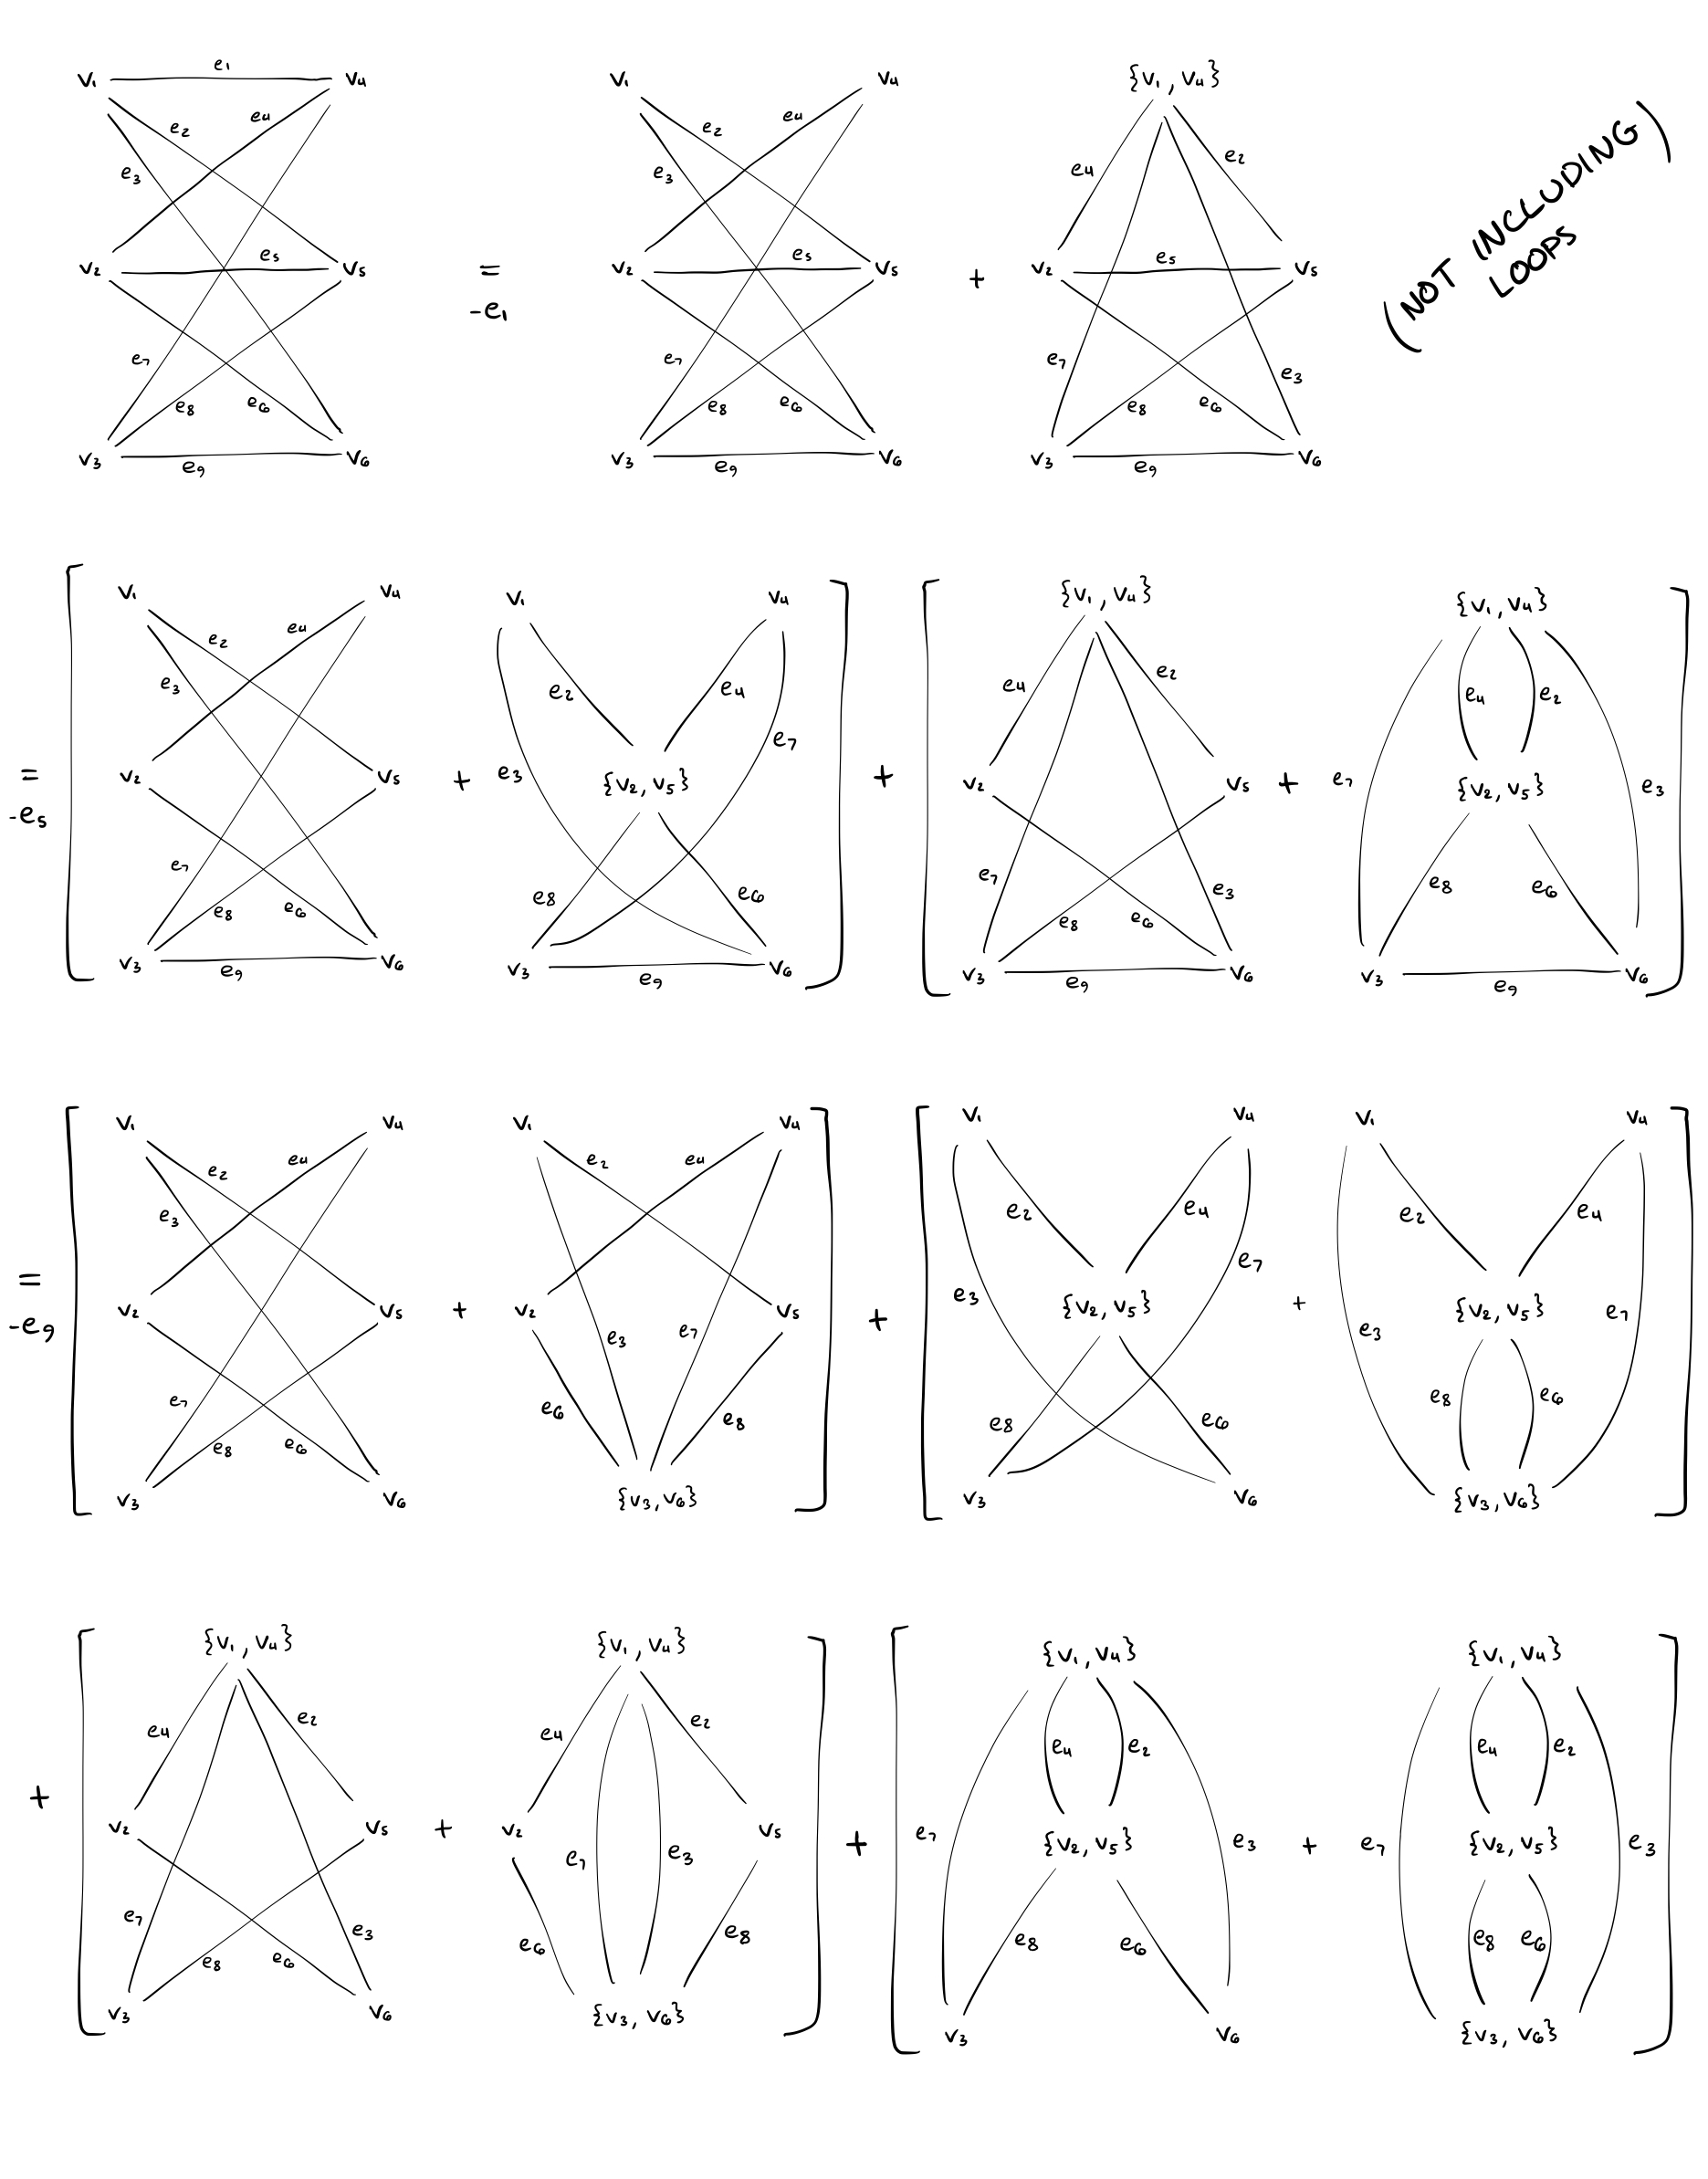
\includegraphics[width=0.95\textwidth]{1.jpeg} \\
  % 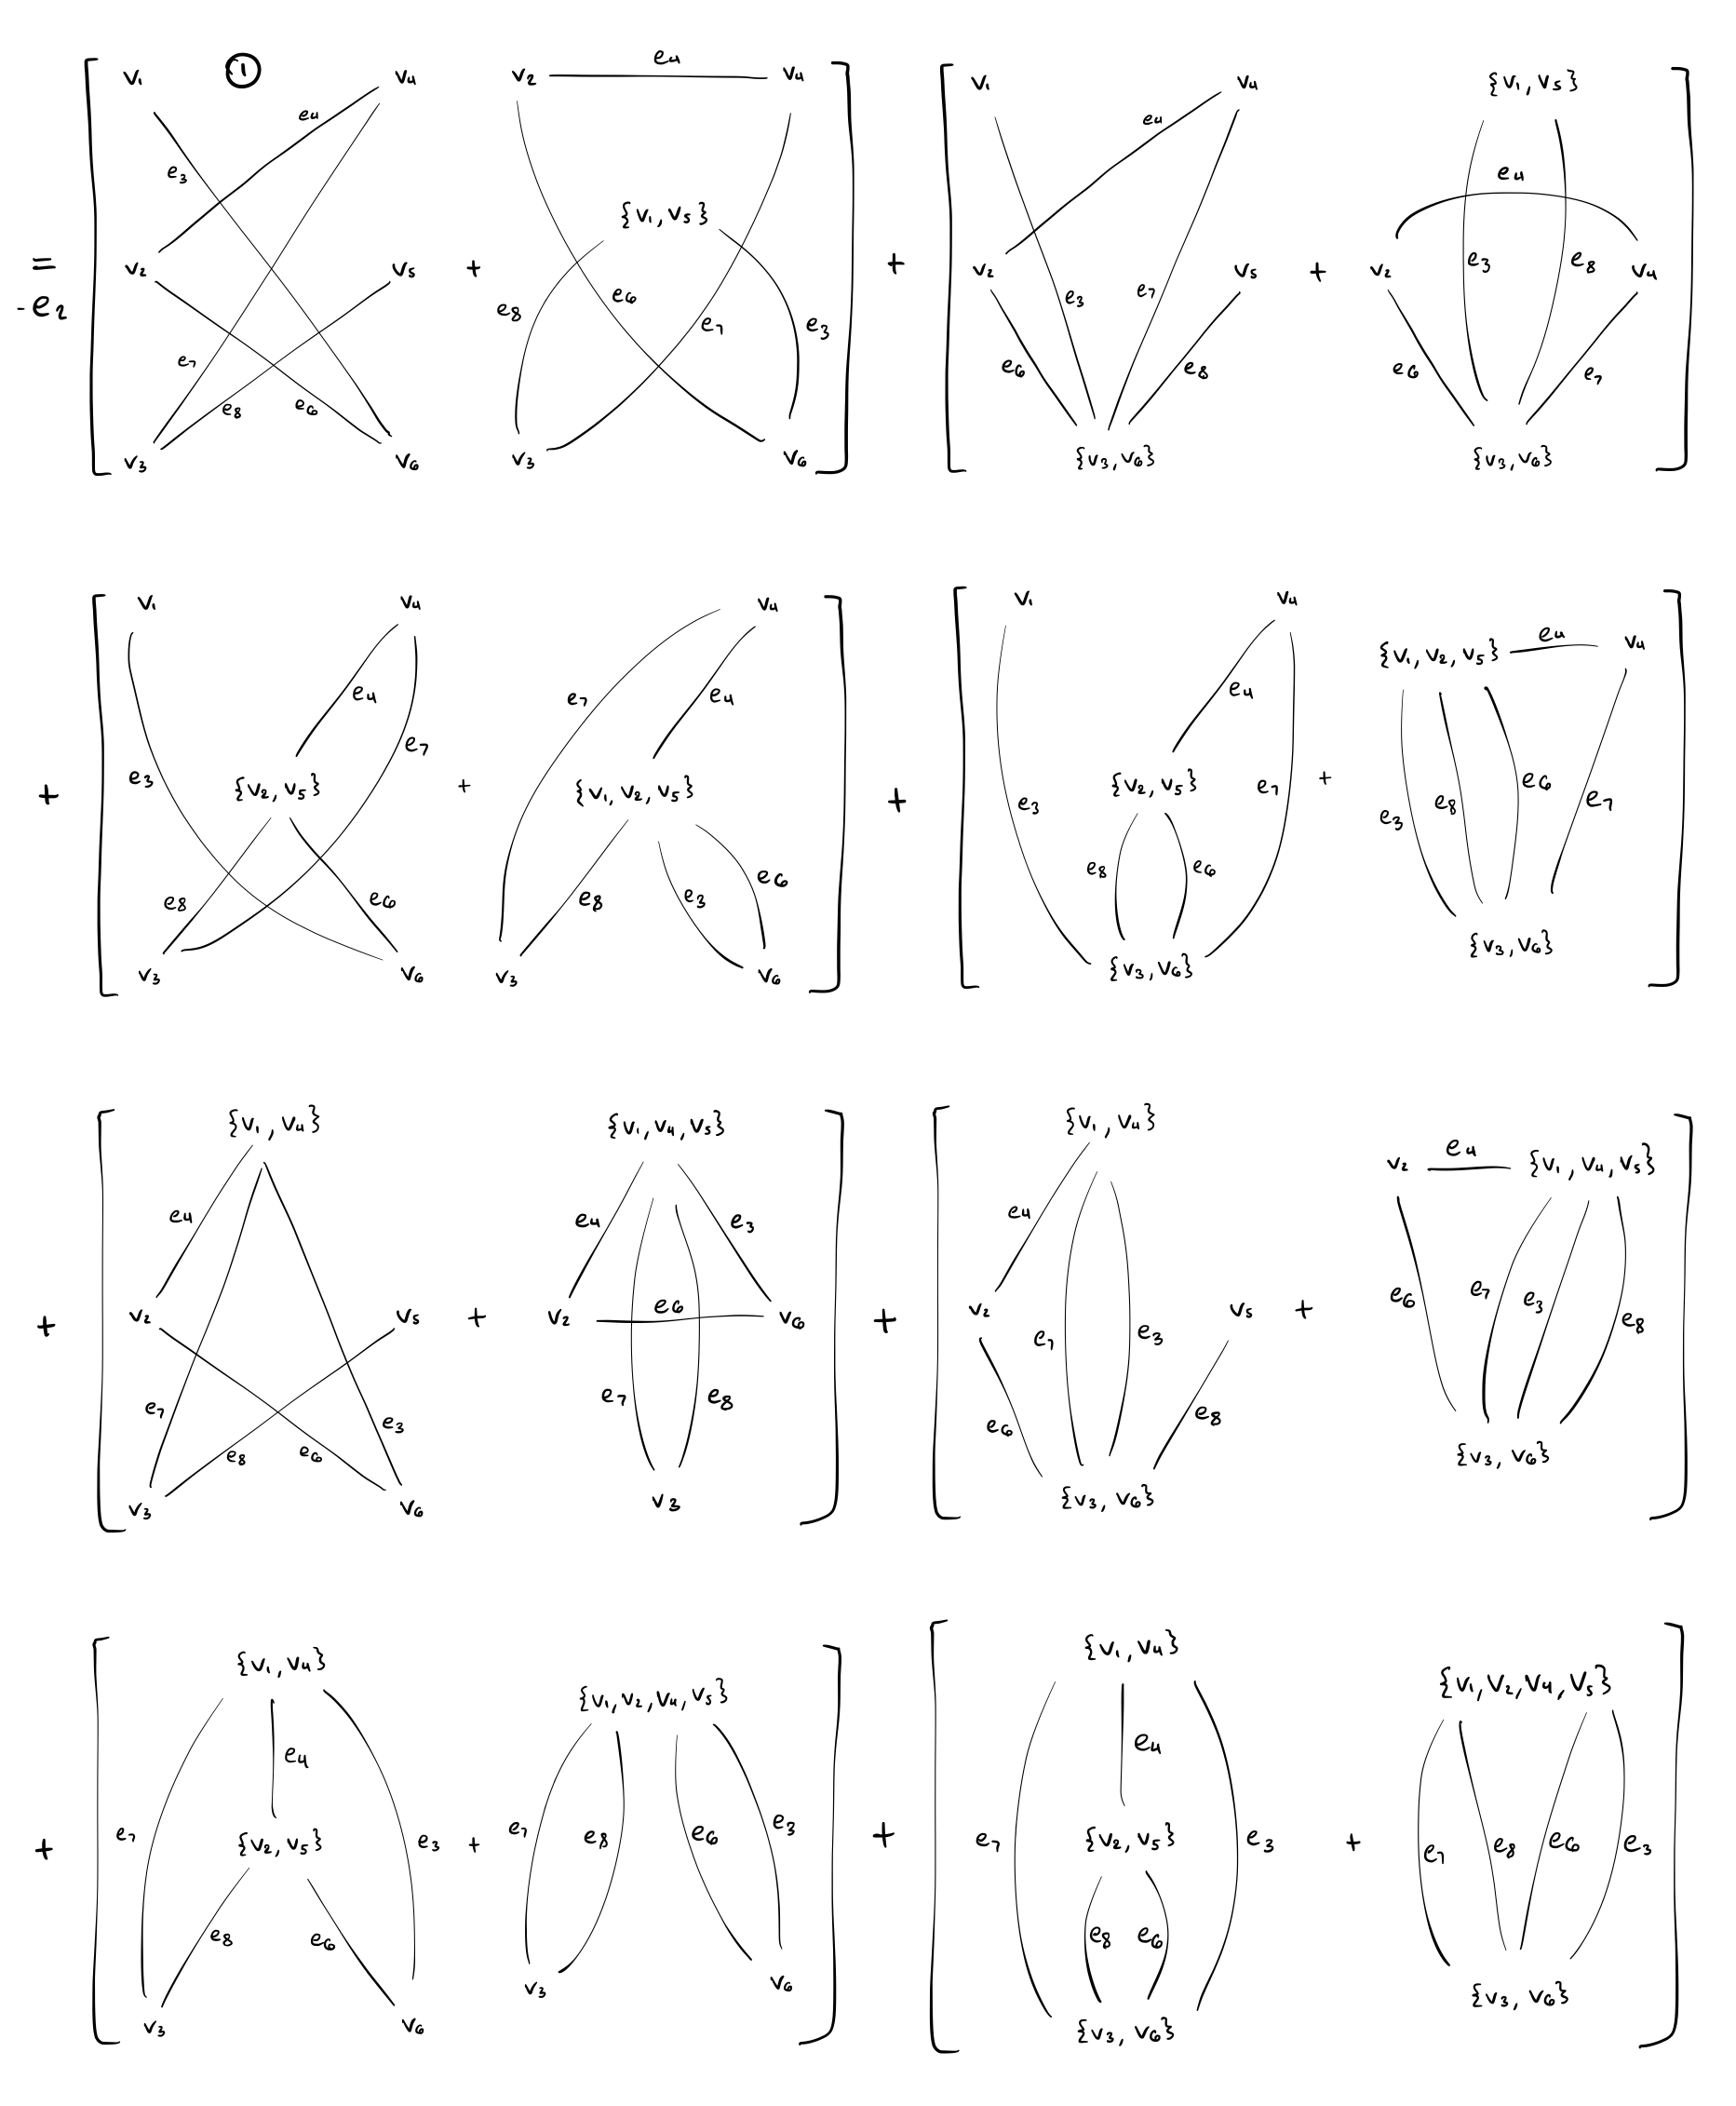
\includegraphics[width=0.95\textwidth]{2.jpeg} \\
  % 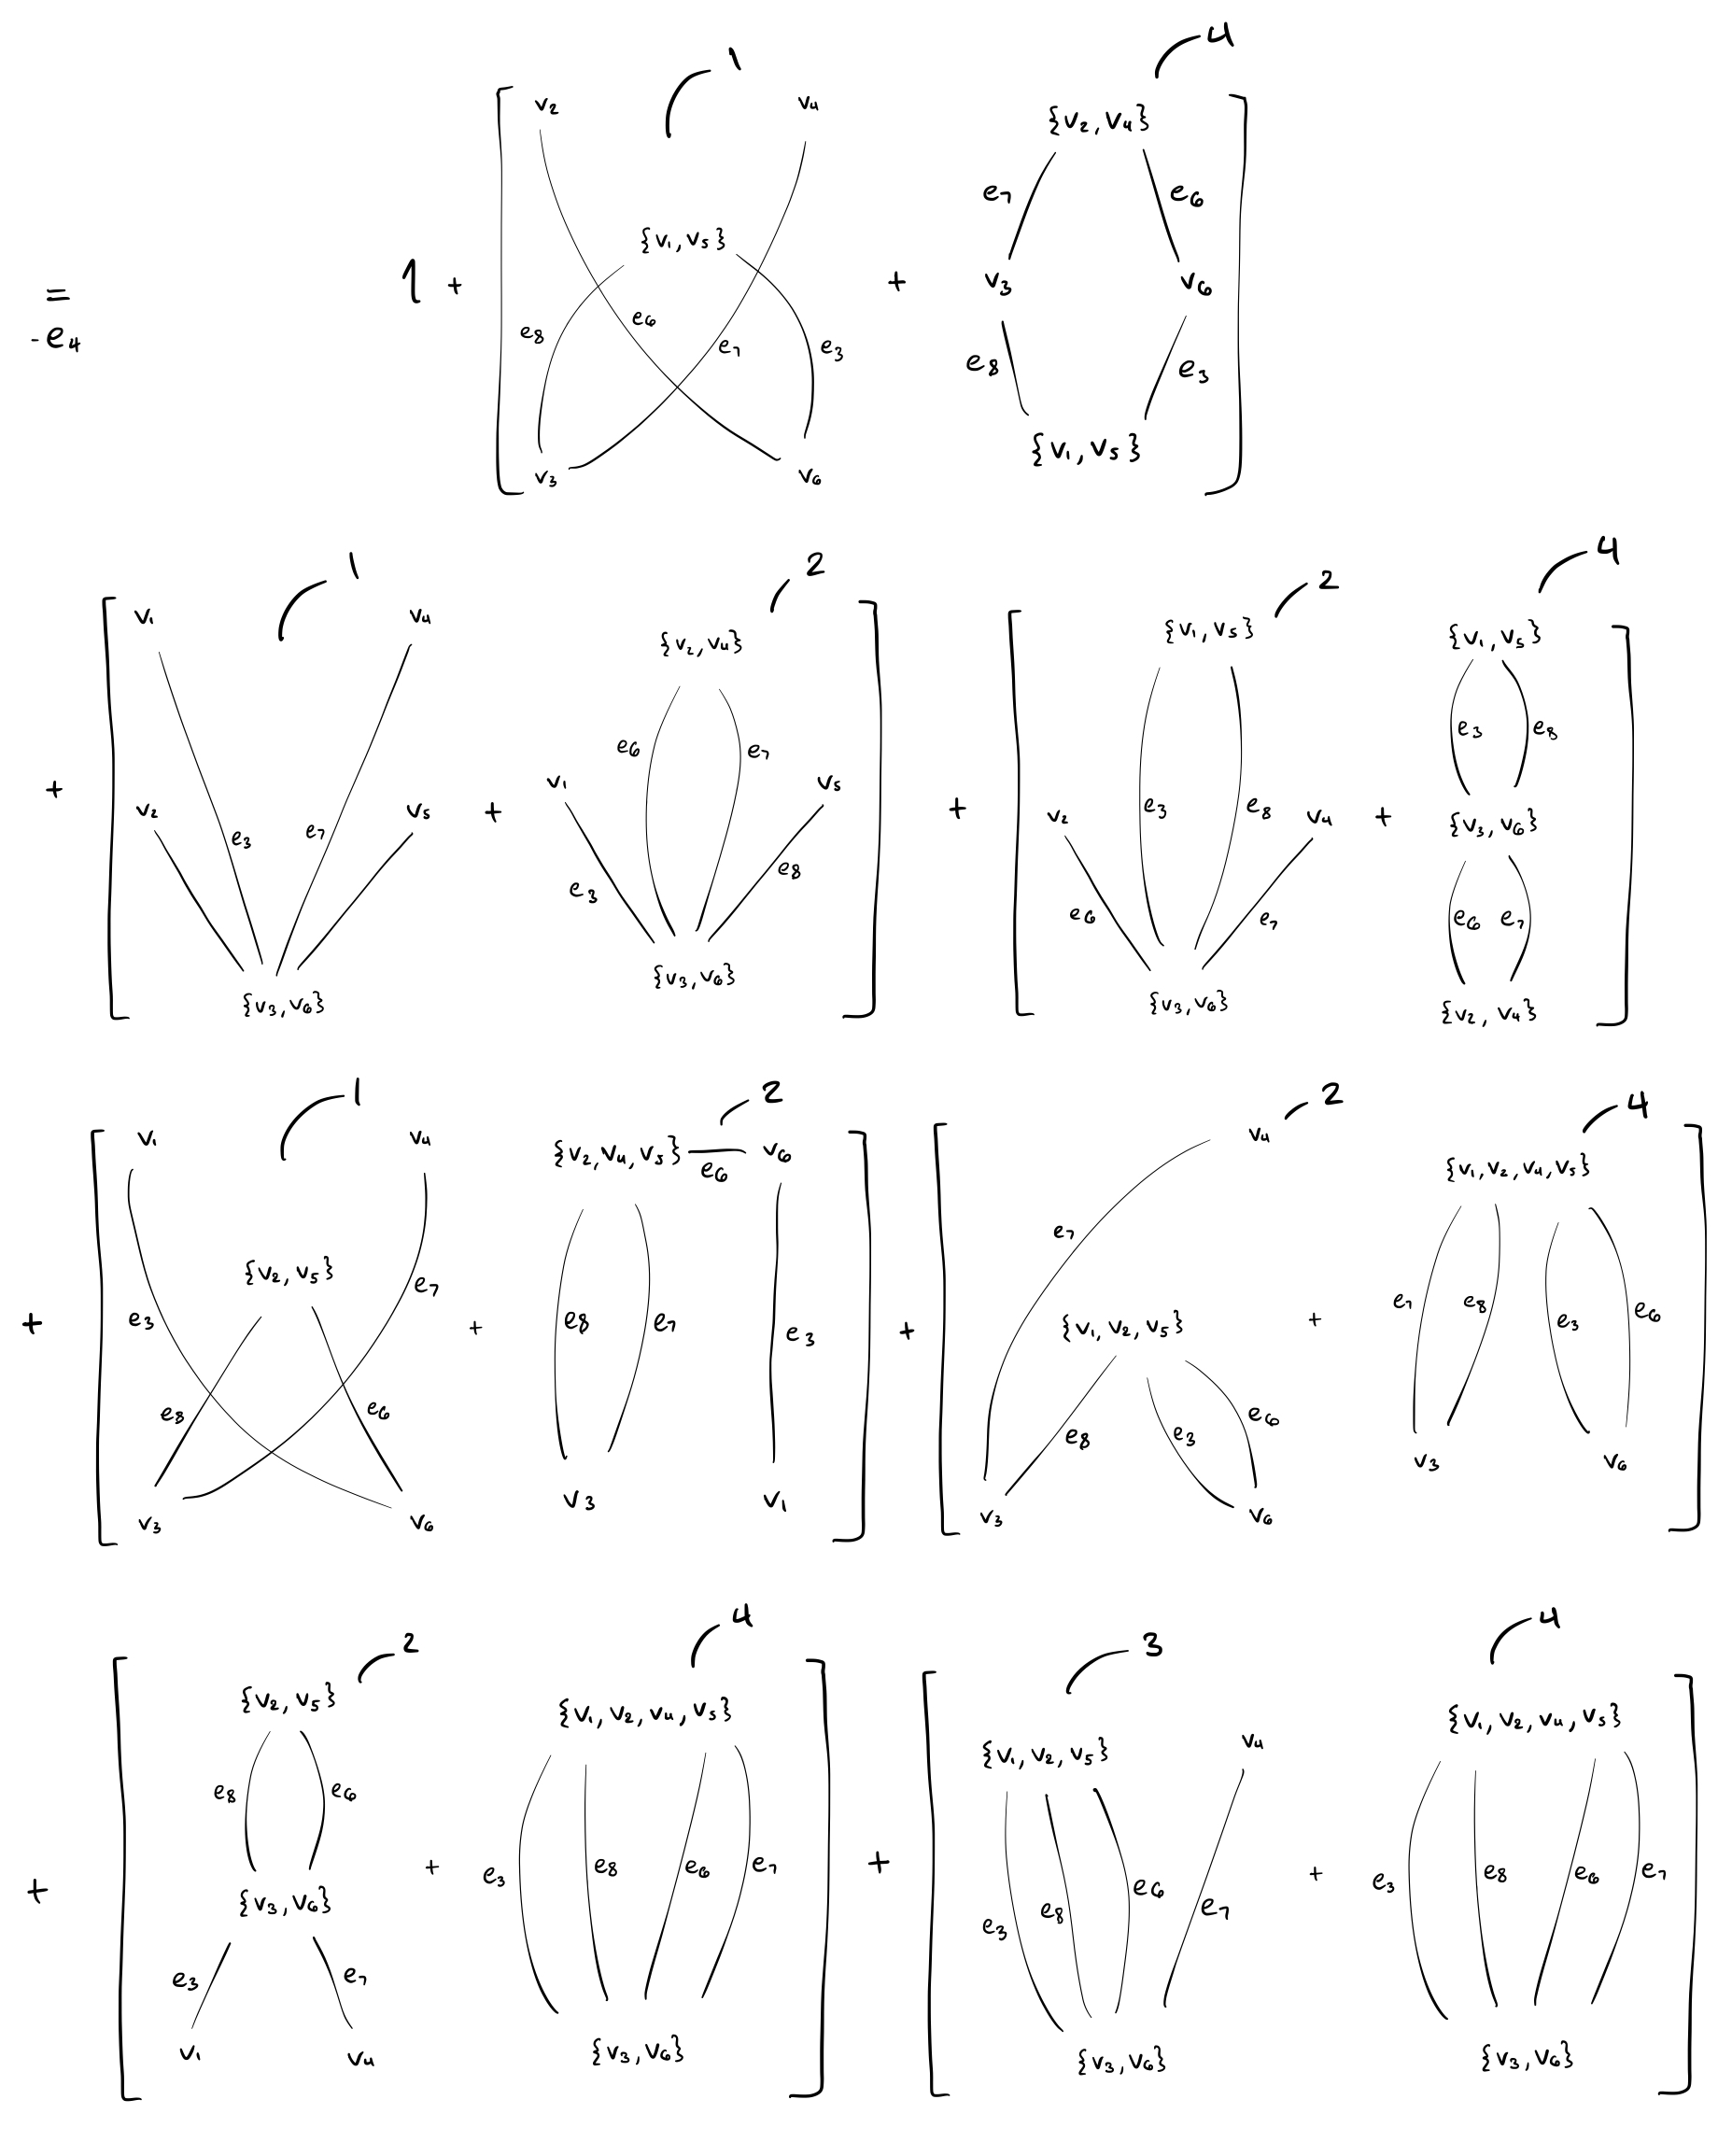
\includegraphics[width=0.95\textwidth]{3.jpeg} \\
  % 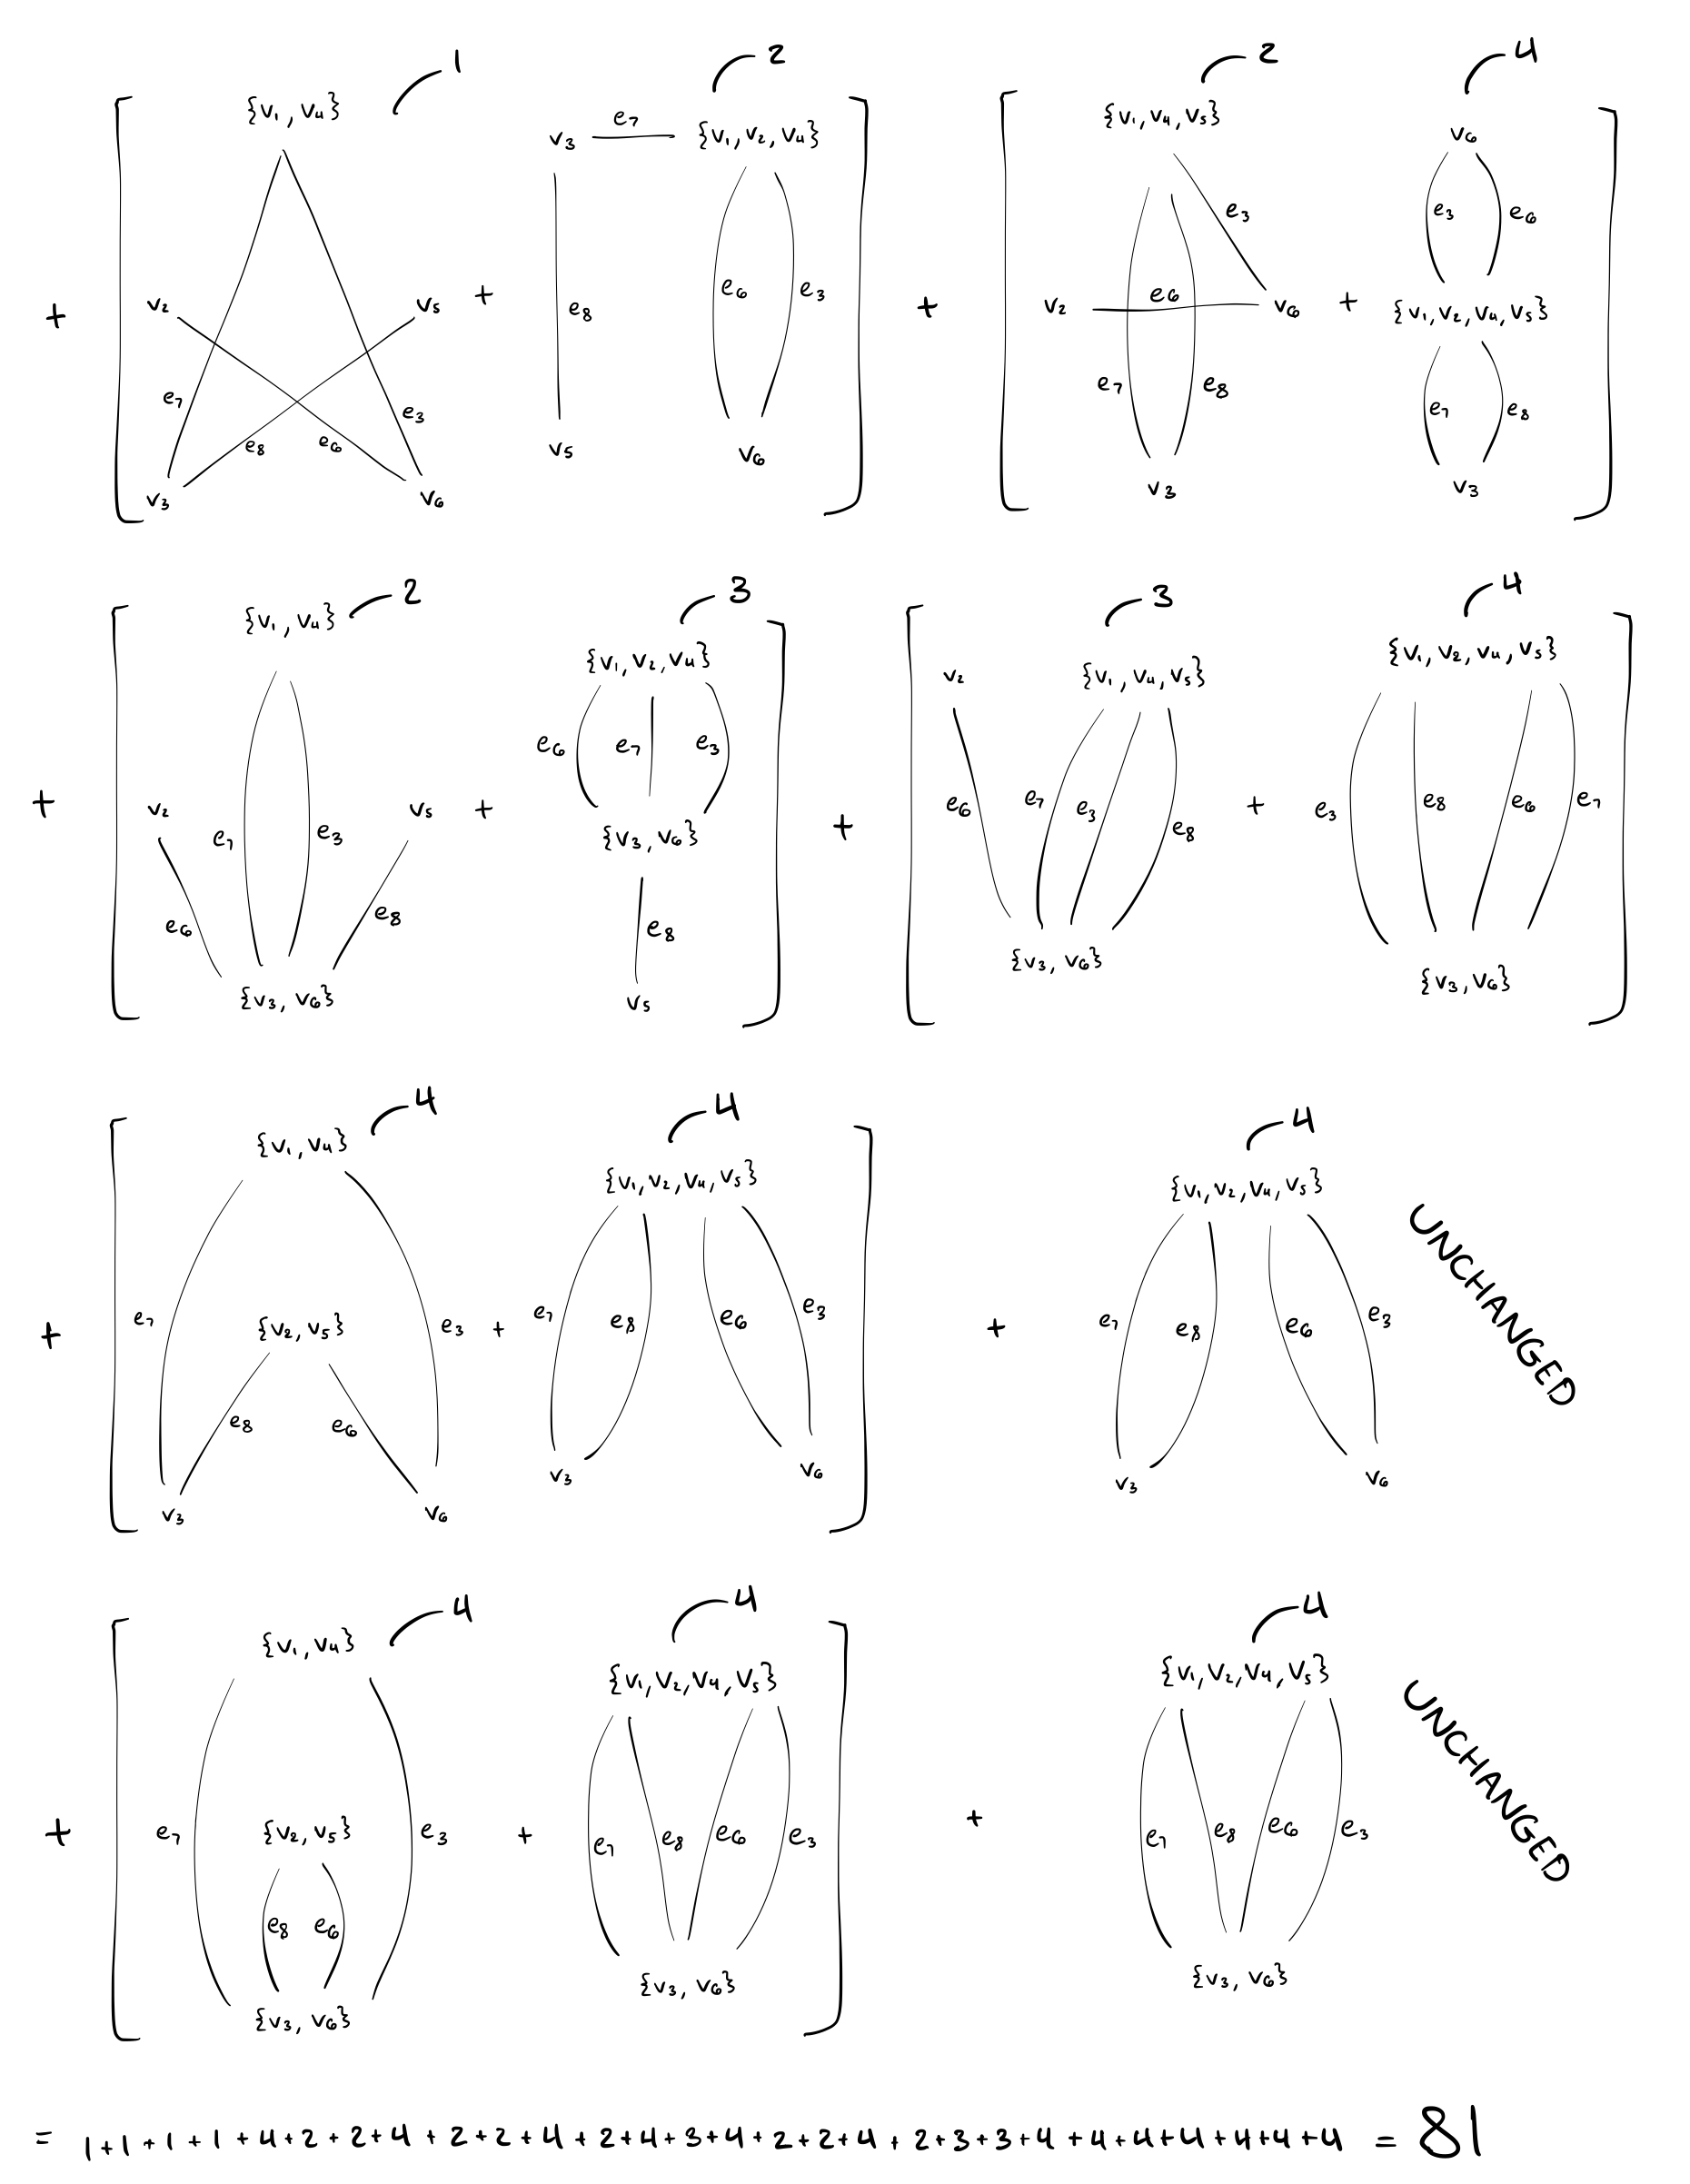
\includegraphics[width=0.95\textwidth]{4.jpeg} \\
  \newpage
  



  \itm{2.4.5} \begin{enumerate}[label=(\alph*)]
      \item Let \(H\) be a graph in which every two adjacent vertices are joined by \(k\) edges and let \(G\) be the underlying simple graph of \(H\).  Show that \(\tau(H) = k^{\nu-1} \tau(G)\).

      \item Let \(H\) be the graph obtained from a graph \(G\) when each edge of \(G\) is replaced by a path of length \(k\).  Show that \(\tau(H) = k^{\varepsilon - \nu + 1} \tau(G)\).

      \item Deduce from (b) tbat \(\tau(K_{2,n}) = n 2^{n-1}\).
    \end{enumerate}



  \itm{2.5.3} Can Kruskal's algorithm be adapted to find
  \begin{enumerate}[label=(\alph*)]
      \item a \textit{maximum}-weight tree in a weighted connected graph?

      \item a minimum-weight maximal forest in a weighted graph?
    \end{enumerate}
    If so, how?



  \itm{2.5.5} The \textit{tree graph} of a connected graph \(G\) is the graph whose vertices are spanning trees \(T_1, T_2, \hdots, T_{\tau}\) of \(G\), with \(T_i\) and \(T_j\) joined if and only if they have exactly \(\nu-2\) edges in common.  Show that the tree graph of any connected graph is connected.



\end{itemize}

\end{document}
